\subsection{Opis hipotezy}\label{opis-hipotezy}

\textbf{Numer:} 7\\\textbf{Nazwa:} Wypadki z udziałem pieszych a
czas\\\textbf{Treść:} Wypadki z udziałem pieszych mogą być częstsze w
weekendy oraz na wiosnę i w lecie, wtedy pieszych na drogach jest
więcej.

\subsection{Wyniki związane z
hipotezą}\label{wyniki-zwiazane-z-hipoteza}

\centerline{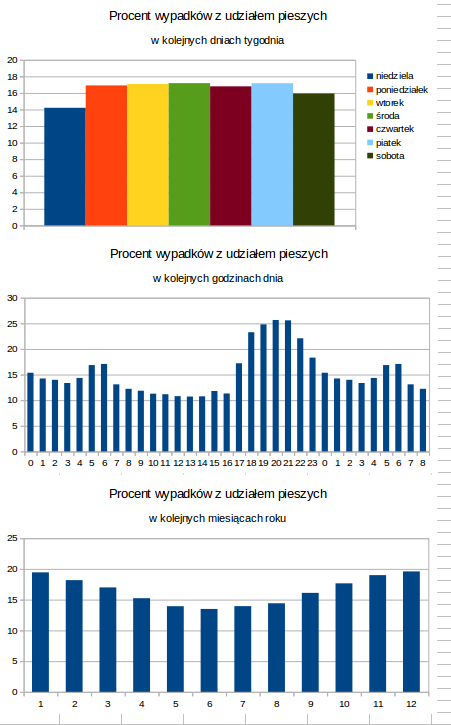
\includegraphics[width=0.8\textwidth]{images/hipotheses/pedestrians/pedestrians.png}}

\subsection{Weryfikacja i wnioski}\label{weryfikacja-i-wnioski}

Hipoteza nie potwierdziła się. Większy udział procentowy wypadków z
udziałem pieszych obserwujemy w ciągu tygodnia od poniedziałku do
piątku. W ciągu roku najmniej wypadków z udziałem pieszych jest właśnie
w miesiącach wakacyjnych (czerwiec, lipiec, sierpień).

Przyczyn takiego stanu rzeczy można szukać np. w fakcie, że jednak ruch
pieszych jest większy poza weekendem, gdyż większość ruchu pieszych to
jednak ludzie udający się do pracy/szkoły. Większy ruch pieszych
sprawia, że i wypadków z ich udziałem jest więcej.

Trudniej wytłumaczyć rozkład wypadków w ciągu roku. Można by się pokusić
o stwierdzenie, że trudniejsze warunki powodują, że wypadków z pieszymi
jest więcej i zgodnie z \href{Hipoteza-2}{hipotezą 2} czasem faktycznie
tak jest, chociaż np. śnieg sprawia, że procentowy udział wypadków z
pieszymi jest mniejszy. Można wskazać ciemność jako jeden z czynników
decydujących - w zimie czy na jesień wcześniej robi się ciemno a w
ciemności obserwujemy wyraźny wzrost procentowego udziału wypadków z
pieszymi.

Analiza wykresu godzinowego może być poparciem tezy o dużym wpływie
ruchu do/z pracy na liczbę wypadków z udziałem pieszych. Największy
procent obserwujemy w godzinach 17-22. Częściowo jest to ruch powrotny z
pracy/szkoły a później ruch związany z wieczornymi wyjściami.
